\documentclass[tikz,border=5pt]{standalone}
\usepackage{graphicx}
\usepackage{xcolor}
\usetikzlibrary{positioning,spy}

% ========================= 用户参数设置 =========================
\definecolor{roi1color}{HTML}{7DA0B4} % ROI 1 颜色 (#7da0b4)
\definecolor{roi2color}{HTML}{1369AF} % ROI 2 颜色 (#1369af)

\newcommand{\samplewidth}{1}
\newcommand{\sampleheight}{1.6}
\newcommand{\magnificationfactor}{2}
\newcommand{\linewidthmacro}{1.5pt}

\begin{document}
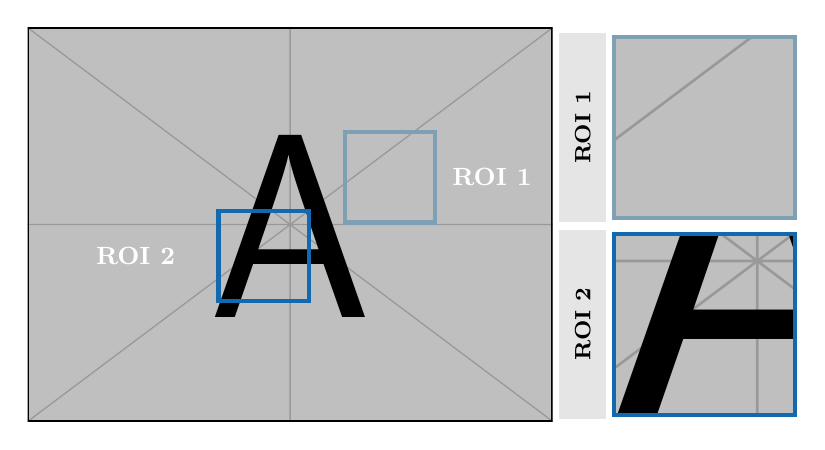
\begin{tikzpicture}[spy using outlines={
    shape=rectangle,
    magnification=\magnificationfactor
}]

% 主图
\node[anchor=south west, inner sep=0] (mainimg) 
  {\includegraphics[height=5cm]{example-image-a}};

% ============= 坐标映射并标注文字 =============
\begin{scope}[x={(mainimg.south east)}, y={(mainimg.north west)}]
  % ROI 1
  \coordinate (spypoint1) at (0.69,0.62);
%   \draw[line width=\linewidthmacro, draw=roi1color] (0.6,0.55) rectangle ++(0.18,0.14);
  \node[anchor=west, text=white, font=\bfseries\small] at (0.79,0.62) {ROI 1};

  % ROI 2
  \coordinate (spypoint2) at (0.45,0.42);
%   \draw[line width=\linewidthmacro, draw=roi2color] (0.36,0.35) rectangle ++(0.18,0.14);
  \node[anchor=east, text=white, font=\bfseries\small] at (0.30,0.42) {ROI 2};
\end{scope}

% % ============= 灰色标签栏 =============
% \draw[fill=gray!20, draw=none] (6.1,0.1) rectangle (6.7,2.4);
% \draw[fill=gray!20, draw=none] (6.1,2.6) rectangle (6.7,4.9);
% \node[rotate=90, text width=1cm, align=center, font=\bfseries\footnotesize] 
%   at (6.4,3.5) {ROI 1};
% \node[rotate=90, text width=1cm, align=center, font=\bfseries\footnotesize] 
%   at (6.4,1) {ROI 2};



% ============= 放大图位置 =============
\node[right=1.8cm of mainimg.north east, anchor=north west, yshift=-1.15cm] (spyviewer1) {};
\node[below=0.9cm of spyviewer1.south west, anchor=north west, yshift=-1.35cm] (spyviewer2) {};

% ============= 放大视图 (独立颜色) =============
\spy[
    width=2.3cm, height=2.3cm,
    draw=roi1color,
    every spy on node/.style={line width=\linewidthmacro, draw=roi1color},
    every spy in node/.style={line width=\linewidthmacro, draw=roi1color}
] on (spypoint1) in node[anchor=center] at (spyviewer1);

\spy[
    width=2.3cm, height=2.3cm,
    draw=roi2color,
    every spy on node/.style={line width=\linewidthmacro, draw=roi2color},
    every spy in node/.style={line width=\linewidthmacro, draw=roi2color}
] on (spypoint2) in node[anchor=center] at (spyviewer2);


% ========== 灰色标签栏(相对定位) ==========
% ROI 1 灰栏节点
\node[left=1.73cm of spyviewer1, anchor=west, fill=gray!20, inner sep=0pt, minimum width=0.6cm, minimum height=2.4cm] (gray1) {};
\node[rotate=90, text width=1cm, align=center, font=\bfseries\footnotesize] at (gray1) {ROI 1};

% ROI 2 灰栏节点
\node[left=1.73cm of spyviewer2, anchor=west, fill=gray!20, inner sep=0pt, minimum width=0.6cm, minimum height=2.4cm] (gray2) {};
\node[rotate=90, text width=1cm, align=center, font=\bfseries\footnotesize] at (gray2) {ROI 2};


\end{tikzpicture}
\end{document}
